\documentclass[a4paper,12pt]{article}
\usepackage[utf8]{inputenc}
\usepackage{csquotes}
\usepackage[T1]{fontenc}
\usepackage[polish]{babel}
\usepackage{xcolor}
\usepackage{graphicx}
\usepackage{amsmath}
\usepackage{amssymb}
\usepackage{hyperref}
\usepackage{float}
\usepackage{listings}
\usepackage[backend=biber, style=numeric]{biblatex}

\addbibresource{bibliografia.bib}

\lstset{
  basicstyle=\ttfamily\small,
  columns=flexible,
  keepspaces=true,
  showstringspaces=false,
  escapeinside={(*@}{@*)},
  literate={ą}{{\k{a}}}1
           {ć}{{\'{c}}}1
           {ę}{{\k{e}}}1
           {ł}{{\l{}}}1
           {ń}{{\'{n}}}1
           {ó}{{\'{o}}}1
           {ś}{{\'{s}}}1
           {ź}{{\'{z}}}1
           {ż}{{\.{z}}}1
           {Ą}{{\k{A}}}1
           {Ć}{{\'{C}}}1
           {Ę}{{\k{E}}}1
           {Ł}{{\L{}}}1
           {Ń}{{\'{N}}}1
           {Ó}{{\'{O}}}1
           {Ś}{{\'{S}}}1
           {Ź}{{\'{Z}}}1
           {Ż}{{\.{Z}}}1
           {"}{{\textquotedbl}}1
           {'}{{\textquotesingle}}1
           {`}{{\textasciigrave}}1
           {~}{{\textasciitilde}}1
           {^}{{\textasciicircum}}1
           {_}{{\textunderscore}}1
           {|}{{\textbar}}1
           {\{}{{\textbraceleft}}1
           {\}}{{\textbraceright}}1
           {[}{{[}}1
           {]}{{]}}1,
  language=SQL,
  showspaces=false,
  numbers=left,
  numberstyle=\tiny,
  commentstyle=\color{green!60!black},
  keywordstyle=\color{blue},
  stringstyle=\color{red!80!black},
  breaklines=true, 
  frame=single,
  captionpos=b 
}

\title{6. sprawozdanie z laboratorium Hurtownie Danych}
\author{Mikołaj Kubś, 272662}
\date{\today}

\begin{document}

\maketitle

\section{Zad. 1. Modyfikacja wymiarów i tabeli faktów}

Bazując na kostce utworzonej przy realizacji listy 4, należy:

\subsection{Podpunkt a}

Zmodyfikować definicję wymiarów tak, aby:

\begin{enumerate}
  \item W wymiarach CUSTOMER i SALESPERSON nie można było korzystać z atrybutów FirstName oraz LastName. W zamian dodać atrybut Names\\
        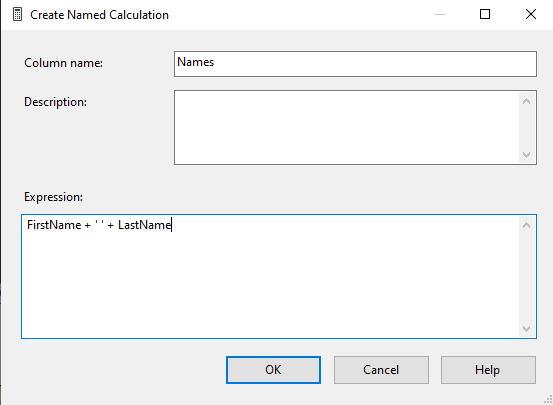
\includegraphics[width=0.6\textwidth]{images/1a1.png}

  \item W wymiarze SALESPERSON pojawiła się hierarchia Group - CountryRegionCode - Names\\
        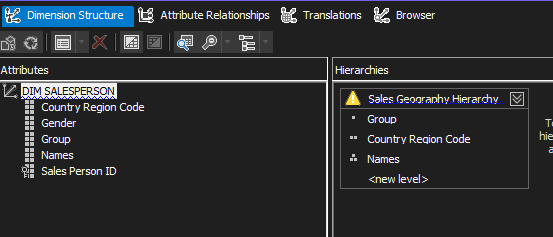
\includegraphics[width=0.6\textwidth]{images/1a2.png}

  \item W wymiarze CUSTOMER pojawiła się hierarchia Group - CountryRegionCode - Names\\
        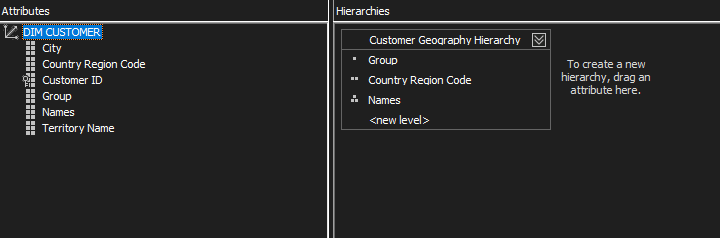
\includegraphics[width=0.6\textwidth]{images/1a3.png}

  \item W wymiarze PRODUCT pojawiła się hierarchia CategoryName - SubCategoryName - Name\\
        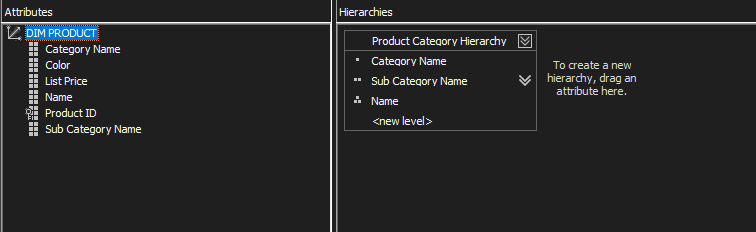
\includegraphics[width=0.6\textwidth]{images/1a4.png}

  \item W wymiarze TIME pojawiła się hierarchia Rok - Kwartał - Miesiąc - Dzień miesiąca\\
        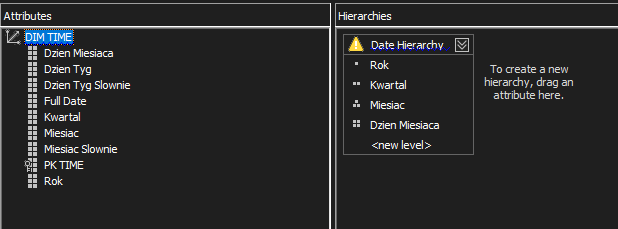
\includegraphics[width=0.6\textwidth]{images/1a5.png}
\end{enumerate}

\subsection{Podpunkt b}

Dla każdego atrybutu kluczowego wymiaru, którego wartościami są liczby całkowite,
zmodyfikować właściwości (Properties). Zmodyfikować parametr NameColumn, tak
aby nazwy kolejnych elementów wymiaru nie były liczbami. (Przykładowo dla wymiaru dotyczącego Produktu można wykorzystać atrybut Name).

\begin{figure}[H]
  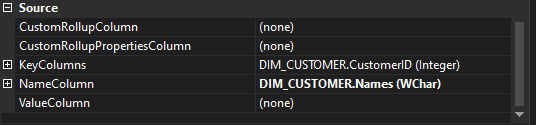
\includegraphics[width=0.6\textwidth]{images/1b_salesperson.png}
  \caption{Widok Properties dla DIM\_Salesperson}
\end{figure}

\begin{figure}[H]
  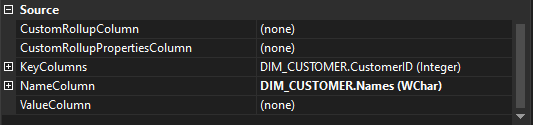
\includegraphics[width=0.6\textwidth]{images/1b_customer.png}
  \caption{Widok Properties dla DIM\_Customer}
\end{figure}

\begin{figure}[H]
  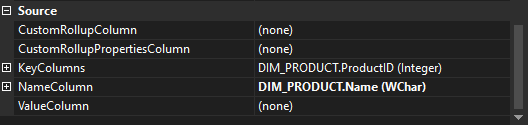
\includegraphics[width=0.6\textwidth]{images/1b_product.png}
  \caption{Widok Properties dla DIM\_Product}
\end{figure}

\begin{figure}[H]
  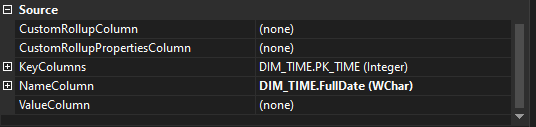
\includegraphics[width=0.6\textwidth]{images/1b_time.png}
  \caption{Widok Properties dla DIM\_Time}
\end{figure}

\subsection{Podpunkt c}

Utworzyć nowe miary, które będą odzwierciedlać:

\begin{itemize}
  \item Liczbę różnych klientów (aggregatedFunction: distinct count)
  \item Liczbę różnych produktów
  \item Maksymalną wartość rabatu (aggregatedFunction: max)
  \item Maksymalną liczbę zamówionych produktów
  \item Liczbę różnych sprzedawców realizujących zamówienia
\end{itemize}

\begin{figure}[H]
  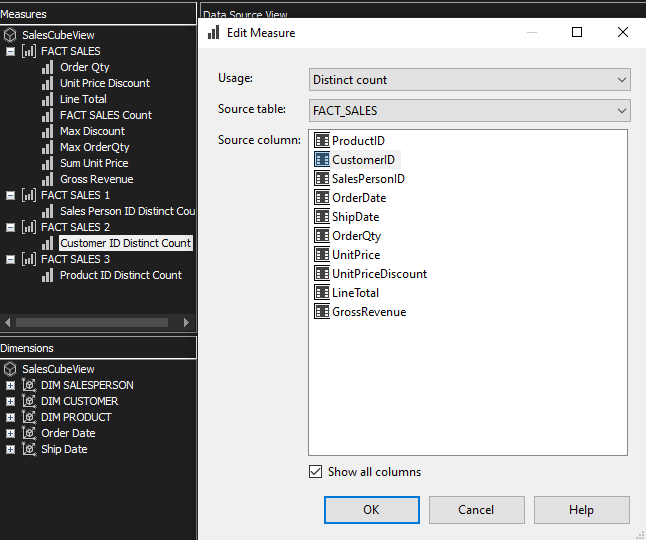
\includegraphics[width=0.6\textwidth]{images/1c.png}
  \caption{Miara dotycząca liczby różnych klientów}
\end{figure}

\subsection{Podpunkt d}

Wdrożyć i przeprocesować kostkę.

\begin{figure}[H]
  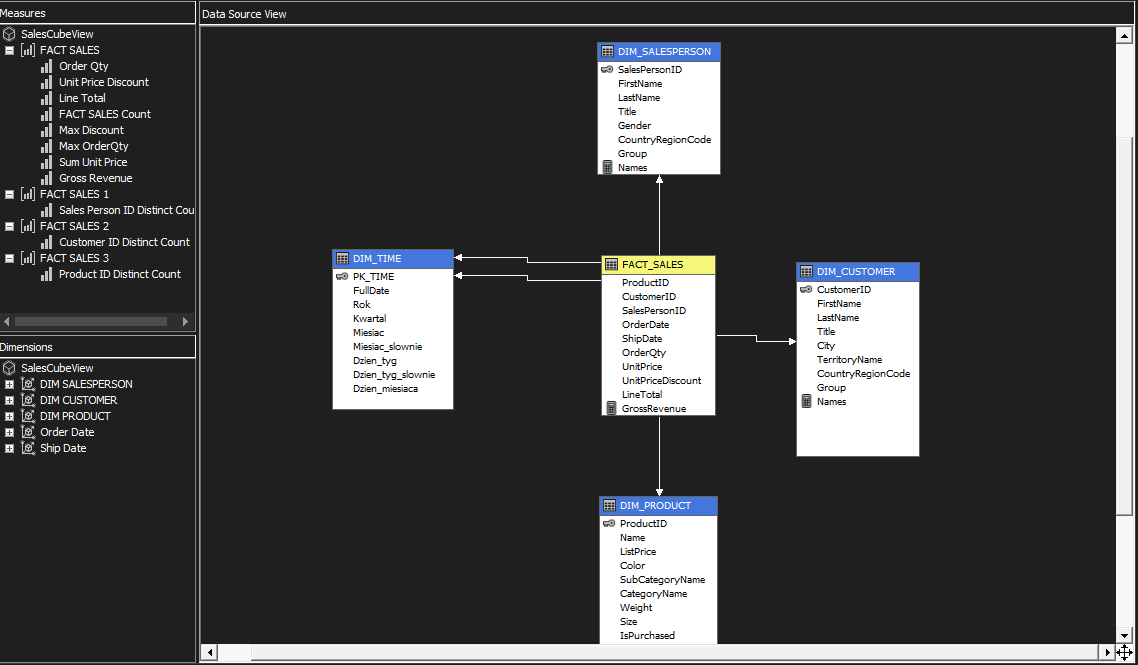
\includegraphics[width=0.6\textwidth]{images/1d.png}
  \caption{Widok przeprocesowanej kostki}
\end{figure}

\section{Zad. 2. Przegląd danych i tworzenie zestawień}

Przy użyciu zakładki Browser:

\subsection{Podpunkt a}

Sprawdzić, czy dane zapisane w kostce zgadzają się z danymi zapisanymi w tabelach, przeciągając za pomocą myszy:
\begin{itemize}
  \item atrybuty wymiarów w region wierszy
  \item miary w część centralną widoku
\end{itemize}

\begin{figure}[H]
  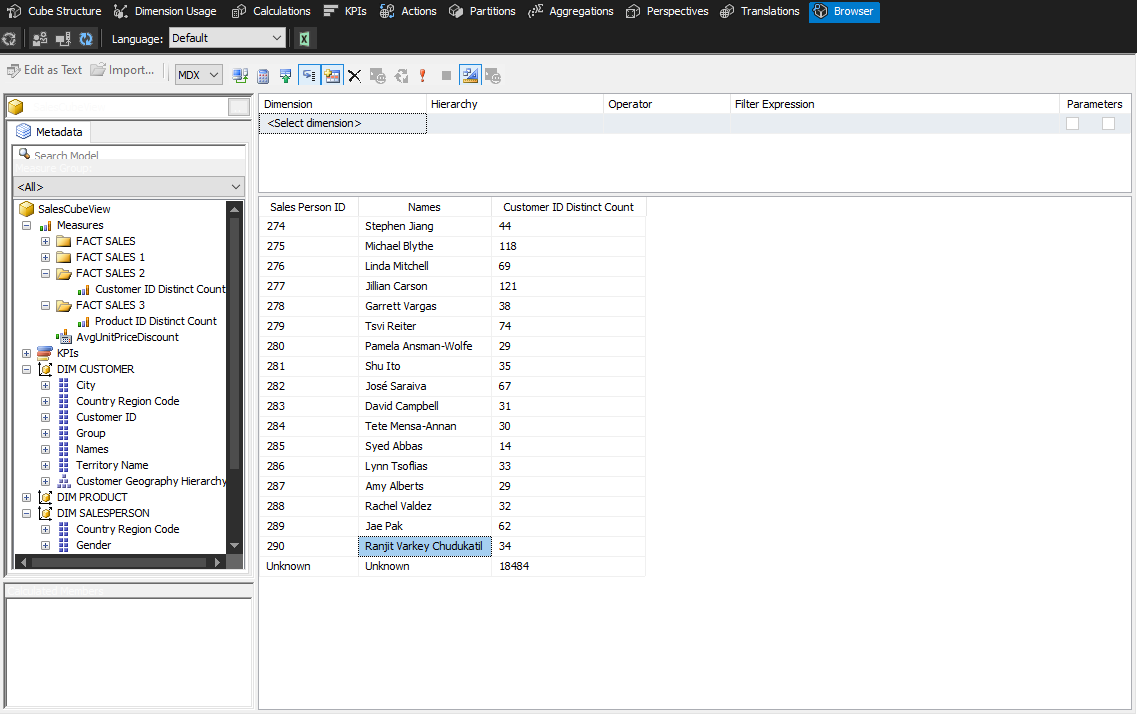
\includegraphics[width=0.6\textwidth]{images/2a.png}
  \caption{Widok przykładowej kwerendy w Browser}
\end{figure}

\subsection{Podpunkt b}

Przetestować możliwości przeglądarki (Browser) - operator wyboru danych (Operator), wyrażenia filtrujące dane (Filter Expression) itp.

\begin{figure}[H]
  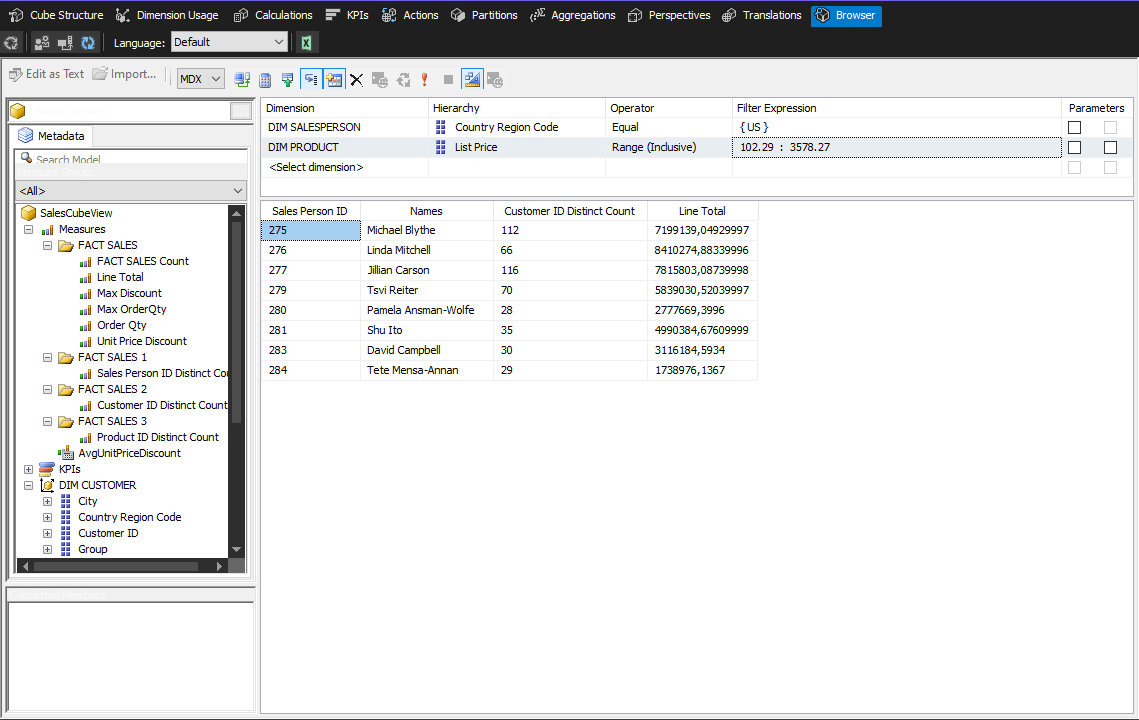
\includegraphics[width=0.6\textwidth]{images/2b.png}
  \caption{Widok przykładowej kwerendy z dwoma różnymi rodzajami filtrów (Operator i Filter Expression)}
\end{figure}

\subsection{Podpunkt c}

Przygotować przykładowe tabele i wykresy przestawne oraz zinterpretować uzyskane
wyniki (proszę zapisać wnioski!)

\subsubsection{Rowery}

\begin{figure}[H]
  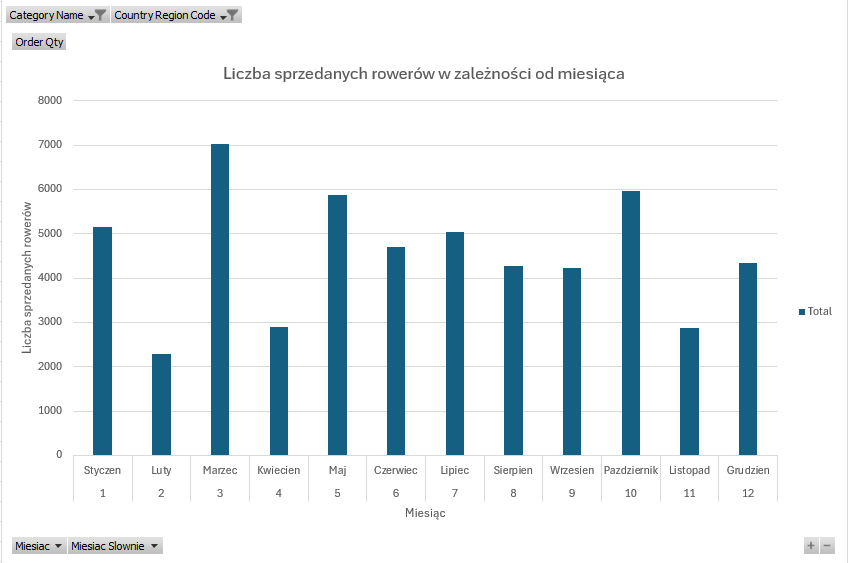
\includegraphics[width=0.6\textwidth]{images/bike_sales.png}
  \caption{Wykres}
\end{figure}

\subsubsection{Rowery}

\begin{figure}[H]
  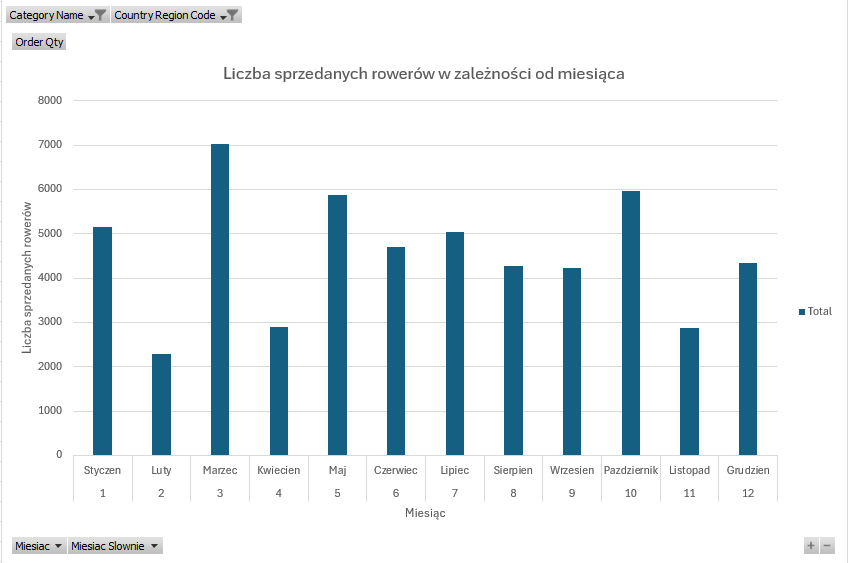
\includegraphics[width=0.6\textwidth]{images/bike_sales.png}
  \caption{Wykres}
\end{figure}

\subsubsection{Zniżka}

\begin{figure}[H]
  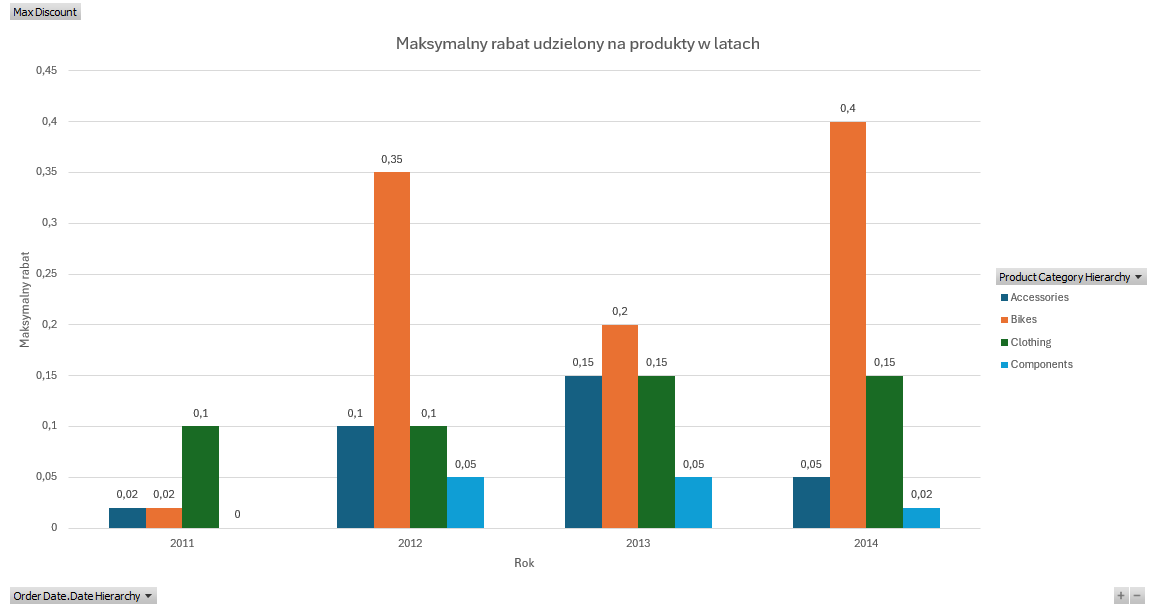
\includegraphics[width=0.6\textwidth]{images/max_discount.png}
  \caption{Wykres}
\end{figure}

\subsubsection{Sprzedawca}

\begin{figure}[H]
  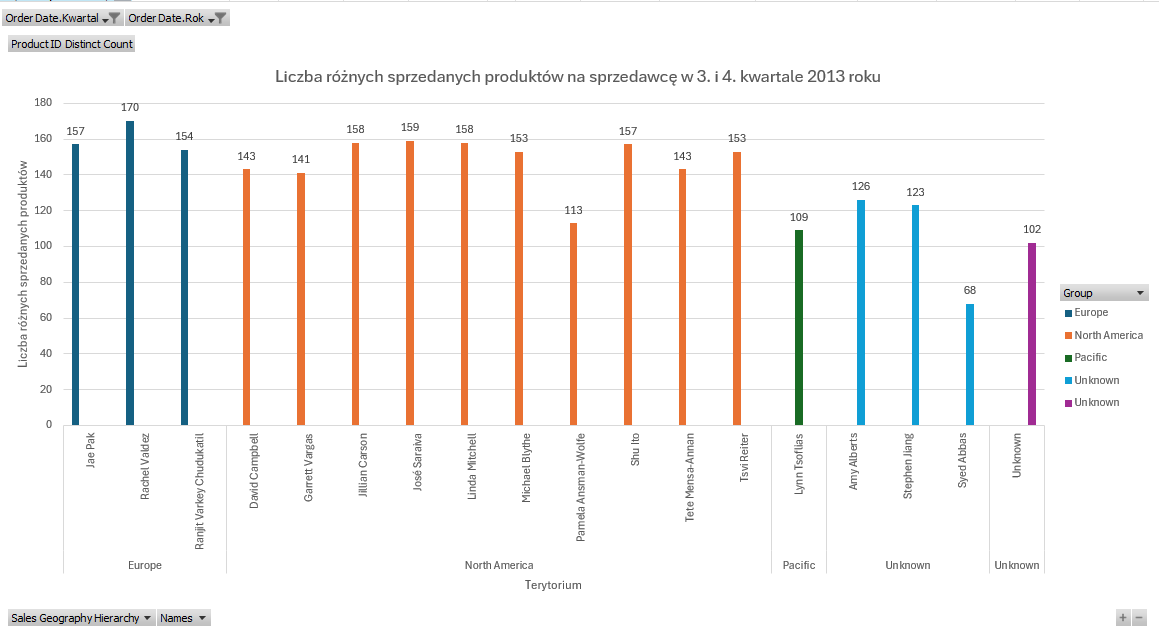
\includegraphics[width=0.6\textwidth]{images/sales_salesperson.png}
  \caption{Wykres}
\end{figure}

\section{Zad. 3. Miary kalkulowane}
\section{Zad. 4. Partycje}
\section{Zad. 5. * Definiowanie KPI}
\section{Wnioski}

\section{Wnioski}

\printbibliography

\end{document}